\documentclass{article}

\usepackage{graphicx}
\usepackage{subfig}
\usepackage{float}
\usepackage{hyperref}
\usepackage{algpseudocode}
\usepackage{mathtools}
\usepackage{amsmath}
\usepackage{amssymb}
\usepackage[utf8]{inputenc}

\title{Biometric Systems}
\author{Eduardo Rinaldi}
\date{}

\begin{document}
\maketitle

\tableofcontents
\newpage

\section{Introduzione}
Il termine ``biometric" deriva dal greco dalle parole ``bios" (\textit{vita}) e ``metron" (\textit{misura}), in informatica questo termine viene usato per descrivere il processo di riconoscimento di una persona tramite \textbf{caratteristiche fisiche} o \textbf{comportamentali}.

\bigskip
Un possibile approccio ai ``Sistemi biometrici" è tramite \textbf{riconoscimento di pattern} (pattern recognition): due pattern $p_1$ e $p_2$ vengono ritenuti simili se e solo se, data una misura di distanza $d$, abbiamo: $d(p_1, p_2) < t$, dove $t$ è una soglia entro la quale la loro distanza deve rientrare. Come possiamo vedere già qui incontriamo i primi problemi riguardanti la scelta di $d$ e $t$.

\bigskip
In generale l'autenticazione di un individuo può avvenire in 3 modi:
\begin{enumerate}
    \item Tramite \textbf{qualcosa che abbiamo} (un oggetto) $\rightarrow$ l'oggetto potrebbe essere rubato
    \item Tramite \textbf{qualcosa che sappiamo} (una password) $\rightarrow$ molto sicuro ma è difficile ricordare tante password
    \item Tramite \textbf{qualcosa che siamo} (un tratto biometrico) $\rightarrow$ facile da usare per l'utente ma non sicuro al 100\%
\end{enumerate}

\subsection{Storia}
L'apripista ai sistemi biometrici fu \textbf{Bertillon} nel 1882, capo della polizia di Parigi che, iniziò a tenere traccia di alcune misure del corpo dei diversi detenuti che gli si presentarono, istituendo pian piano così il primo sistema di riconoscimento biometrico. Il sistema fu poi criticato su un punto di vista statistico da parte di \textbf{Galton}, quest'ultimo invece, introducendo il concetto di ``minuzie", fu il pioniere del riconoscimento tramite impronte digitali.

\subsection{Architettura di un sistema biometrico}
Un sistema biometrico può essere suddiviso in principalmente due fasi:
\begin{enumerate}
    \item \textbf{Enrollment}: avviene la cattura del dato biometrico e viene poi processato andando a estrarne le feature, creando così il template; questo viene poi salvato all'interno di una ``gallery" (che possiamo vedere come un database).
    \item \textbf{Riconoscimento}: avviene la cattura del dato biometrico e la conseguente creazione del template, proprio come nella fase di enrollment, poi successivamente questo viene confrontato con altri template nella gallery. Il processo di confronto può essere di due tipi: 
    \begin{itemize}
        \item \textbf{Verifica}: l'utente reclama una certa identità e il sistema deve verificarla (1:1)
        \item \textbf{Identificazione}: il sistema deve identificare da solo l'identità dell'utente tra tutti quelli nella ``gallery" (1:N). Può a sua volta dividersi in ``\textbf{open-set}" (i template in input possono non essere presenti nella gallery) e ``\textbf{closed-set}".
    \end{itemize}
\end{enumerate}

Da qui in avanti per \textbf{probe} intenderemo ogni template dato "in pasto" al sistema per la fase di riconoscimento.

\paragraph{Tipi di utente} cooperativi/non-cooperativi, abituati/non abituati, pubblico/privato, consapevole/non consapevole.

\subsubsection{Tratti biometrici}
Ogni tratto biometrico deve avere le seguenti proprietà:
\begin{itemize}
    \item \textbf{Universalità}: chiunque (o quasi) può averlo
    \item \textbf{Unicità}: è diverso per ogni individuo
    \item \textbf{Permanenza}: non cambia negli anni
    \item \textbf{Misurabilità}: deve poter essere misurabile da un sensore
    \item \textbf{Accettabilità}: gli utenti coinvolti non devono essere contrari alla raccolta di dati per quel tratto
\end{itemize}

Definiamo come ``tratti biometrici \textbf{strong}" quelli che hanno le proprietà sopra citate, alcuni esempi sono: 
\begin{itemize}
    \item \textbf{Tratti fisici}: impronte digitali, occhi (iride e sclera), faccia, orecchie, mani
    \item \textbf{Tratti comportamentali}: camminata, firma
    \item \textbf{Mixed}: voce
    \item \textbf{Biologici}: DNA
\end{itemize}

Definiamo, invece, come ``tratti biometrici \textbf{weak}" quelli che al contrario non sono sufficienti ad identificare una persona da un'altra (es.: il colore dei capelli).

\bigskip
I sistemi biometrici portano un grande vantaggio per quanta riguarda la facilità di utilizzo per un utente (basti pensare allo sblocco del telefono tramite face-id rispetto a uno tramite PIN), ma bisogna tenere bene a mente gli aspetti negativi come: 
\begin{itemize}
    \item la non affidabilità al 100\%
    \item la non usabilità da parte di alcuni utenti
    \item il cambio di alcuni tratti con il passare degli anni
    \item il sistema biometrico potrebbe non essere utilizzabile in alcuni momenti (es.: face-id con la mascherina per il Covid)
\end{itemize}

\section{Valutazione delle performance}
In un sistema biometrico è molto importante effettuare una fase di valutazione delle performance del modello, in quanto da questa possiamo ricavare informazioni utili riguardo a esso. Si possono presentare i seguenti problemi/casi:
\begin{itemize}
    \item Una variazione intra-classe molto alta $\rightarrow$ vedendo i sample come punti in uno spazio possiamo dire che quelli della stessa classe sono molto distanti tra loro
    \item Una variazione inter-classe molto bassa $\rightarrow$ sample tra classi diverse sono molto vicini tra loro
    \item Acquisizione distorta o con ``rumore" (\textit{noise})
    \item Attacchi in diversi punti del sistema biometrico (\textit{spoofing})
\end{itemize}

\subsection{Errori in fase di verifica}
Nella fase di verifica, un soggetto viene accettato se e solo se la distanza tra il probe e i template associati all'identità reclamata è minore o uguale di una certa soglia (\textit{threshold}). Quindi si possono presentare 4 output:
\begin{itemize}
    \item Accettazione ``genuina" (\textbf{Genuine acceptance - GA}): l'identità reclamata è vera e il soggetto viene accettato dal sistema.
    \item Rifiuto ``errato" (\textbf{False rejection - FR}): l'identità reclamata è vera e il soggetto viene rifiutato dal sistema. (\textit{type I})
    \item Accettazione ``errata" (\textbf{False acceptance - FA}): l'identità reclamata è falsa e il soggetto viene accettato dal sistema. (\textit{type II})
    \item Rifiuto ``genuino" (\textbf{Genuine rejection - GR}): l'identità reclamata è falsa e il soggetto viene rifiutato dal sistema.
\end{itemize}

Diverse misure di valutazione possono essere utilizzate, le principali sono:
\begin{itemize}
    \item \textbf{FA Rate}: probabilità di un impostore di essere accettato dal sistema. Viene calcolato dalla seguente formula (semplificata) $$FAR(t) = \frac{|\{\text{probe di soggetti impostori accettati}\}|}{|\{\text{probe di soggetti impostori}\}|}$$ (Da notare che i soggetti impostori potrebbero non essere nella gallery, ma potrebbero anche essere nella gallery e fanno un claim ``da impostore")
    \item \textbf{FR Rate}: probabilità di un utente "genuino" di essere rifiutato dal sistema. Viene calcolato dalla seguente formula (semplificata) $$FRR(t) = \frac{|\{\text{probe di soggetti con claim genuino ma rifiutati}\}|}{|\{\text{probe di soggeti con claim genuino}\}|}$$ (Da notare qui che i soggetti presi in considerazione sono solo quelli nella gallery)
\end{itemize}

Da questi possiamo derivare:
\begin{itemize}
    \item $GAR = 1 - FRR$
    \item $GRR = 1 - FAR$
    \item $EER: FAR = FRR$
    \item Detection Error Trade-off (\textbf{DET}): mette in relazione FAR e FRR
    \item Receiving Operating Characteristics (\textbf{ROC}): mette in relazione 1-FRR (GAR) e FAR
\end{itemize}

\subsection{Errori in fase di identificazione - Open-set}
L'obiettivo del sistema è quello di verificare se il soggetto è all'interno del database e in tal caso capire chi è (senza alcun ``claim" di identità da parte dell'individuo). Rispetto alla fase di verifica si presentano casi diversi:
\begin{enumerate}
    \item Ci sono individui nel database che superano la soglia di accettazione $\And$ l'identità associata al template a rango 1 è quella corretta $\rightarrow$ \textit{corretta identificazione}
    \item Non ci sono individui nel database che superano la soglia di accettazione $\rightarrow$ \textit{identificazione errata}
    \item Ci sono individui nel database che superano la soglia di accettazione $\And$ l'identità associata al template a rango 1 è errata $\rightarrow$ \textit{identificazione errata}
\end{enumerate}

Le misure di valutazione che possiamo utilizzare sono le seguenti:
\begin{itemize}
    \item Detect e Identification rate (\textbf{DIR}) a rango $k$: probabilità di avere una corretta identificazione entro il rango $k$. Possiamo calcolarlo dalla seguente formula:
    $$DIR(t,k) = \frac{| \{ p_j : rango(p_j) \leq k \land d_{i,j} \leq t \land id(p_j) = id(g_i) \}|}{|P_G|}$$
    \item \textbf{FRR}: 1 - DIR(t, 1)
    \item \textbf{FAR}: è definito dal rapporto tra il numero di volte un probe non presente nella gallery supera la soglia di accettazione e il numero di probe non presenti nella gallery che sono stati testati
    $$FAR(t) = \frac{|\{p_j : max_i\ d_{i,j} \leq t \}|}{|P_N|},$$ $\forall p_j \in P_N$ e $\forall g_i \in G$
\end{itemize}
Da questi è poi possibile ottenere altre metriche come:
\begin{itemize}
    \item EER
    \item ROC, questa volta vengono messi in relazione $FAR(t)$ e $DIR(t, 1)$
\end{itemize}

In base all'applicazione finale ovviamente vanno scelte le metriche a cui dare maggior rilevanza:
\begin{itemize}
    \item Se volessimo un'applicazione con pochi falsi allarmi (FAR basso), dovremmo scendere a compromessi sulla misura DIR
    \item Se volessimo un'applicazione in cui è più importante un'identificazione corretta invece, dovremmo scendere a compromessi sulla misura FAR
\end{itemize}

\subsection{Errori in fase di identificazione - Closed-set}
L'identificazione closed-set è un caso speciale in cui si assume che il soggetto associato a ogni probe ha sicuramente una corrispondenza nella gallery. Questo caso, seppur applicabile in pochi contesti, va comunque tenuto in considerazione. Possiamo utilizzare le seguenti metriche:
\begin{itemize}
    \item Cumulative Match Score a rango $k$ ( \textbf{CMS(k)} ): probabilità di identificare un soggetto entro il rango $k$
    \item Cumulative Match Characteristic (\textbf{CMC}): curva che mostra per ogni rango $k$ il valore $CMS(k)$.
    \item Recognition Rate (\textbf{RR}): $CMS(1)$
\end{itemize}

\subsection{Organizzazione del dataset}
Una cosa da tenere bene a mente è che in fase di sviluppo e test del modello noi abbiamo sempre a disposizione il ``\textit{ground truth}" di ogni template, nel momento in cui invece un modello viene utilizzato poi in situazioni reali, questa informazione è ovviamente non disponibile.

\bigskip
Per una buona valutazione di un sistema è molto importante avere una buona suddivisione del dataset. Questa avviene su diversi livelli.

\paragraph{Suddivisione TR vs TS} Anche se non è richiesto alcun procedimento di ``\textit{training}" in senso lato ML, bisogna comunque suddividere il dataset in ``\textit{train}" e ``\textit{test}" set in quanto potrebbe essere necessario effettuare il tuning di qualche parametro (es.: una normalizzazione). L'obiettivo qui è quello di consentire una fase di training che possa generalizzare, e quindi vedere, esempi molto differenziati tra loro. E' possibile inserire in \textbf{TS} template di soggetti che non appaiono completamente in \textbf{TR}, così che si possa testare una maggiore generalizzazione del modello. $TR \cap TS = \emptyset$ è fondamentale.

\paragraph{Suddivisione probe vs gallery}
Questa suddivisione viene effettuata per sample, una condizione fondamentale è $P \cap G = \emptyset$.
E' buona norma inserire nella gallery i template catturati in condizioni controllate, in quanto nella realtà è la condizione più frequente.

\paragraph{Suddivisione probe set} Questa suddivisione è fatta per soggetto e può essere di due tipi:
\begin{itemize}
    \item $P = P_G \cup P_N$
    \item $P = P_G$
\end{itemize}
Il primo caso potrebbe condizionare i risultati di valutazione nel caso di identificazione open-set.

\bigskip
Un modo per diminuire il bias in fase di valutazione è quello di ripetere la valutazione con differenti combinazioni di training e test set per poi effettuarne la media. Un possibile approccio è dato dal \textbf{K-Fold cross validation}.

\subsection{All probe vs All gallery}
E' possibile calcolare da subito una matrice di distanze tra coppie di template probe-gallery e può essere utilizzata per la valutazione di diversi tipi di applicazioni. Ogni riga corrisponde a un'operazione di riconoscimento su un probe in input.

\bigskip 
Il problema di questo approccio è che i risultati dipendono molto dalla suddivisione ``\textit{probe vs gallery}", in quanto forniscono ognuna una matrice di distanze diversa e quindi bisogna effettuare un numero sufficiente di test.

\subsection{All vs All}
Un metodo alternativo al precedente consiste nel calcolare una matrice di distanze tra tutti i possibili template, ognuno dei quali giocherà entrambi i ruoli di ``probe" e ``gallery template". Ogni probe (quindi ogni riga) potrà a turno essere considerato impostore o genuino.

Analizziamo pro e contro:
\begin{itemize}
    \item Pro: facile da programmare e mette sotto stress il sistema in quanto ci saranno molti più tentativi da impostore rispetto a quelli da ``genuino".
    \item Contro: il calcolo della matrice può essere dispendioso e non è possibile creare delle distribuzioni particolari tra probe e gallery, le quali potrebbero fornire dei risultati interessanti.
\end{itemize}

Di seguito vengono riportati gli algoritmi per i possibili tipi di operazione; hanno in comune i seguenti elementi:
\begin{itemize}
    \item M = matrice delle distanze
    \item N = numero di soggetti
    \item G = numero totale di sample = numero di righe/colonne di M
    \item S = numero di template per soggetto ($|G| = S x N$)
    \item i = indice righe, j = indice colonne
    \item $label(x) $ = verà identità di x
\end{itemize}

\bigskip
\paragraph{Verifica, template singolo} ogni riga è un set di $|G|-1$ operazioni, con $S-1$ test genuini e $(N-1)\times(S)$ test da impostore.

\begin{figure}[H]
    \centering
    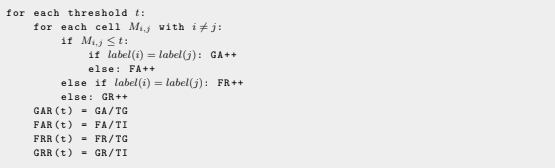
\includegraphics[width=5in]{imgs/verifica-st.PNG}
    \caption{}
    \label{fig:verifica-st}
\end{figure}
Dove \textit{TG} è il numero totale di tentativi genuini e \textit{TI} è il numero totale di impostori.


\paragraph{Verifica, template multipli} ogni riga è un set di $N$ operazioni, con 1 test genuino e $N-1$ test da impostore.

\begin{figure}[H]
    \centering
    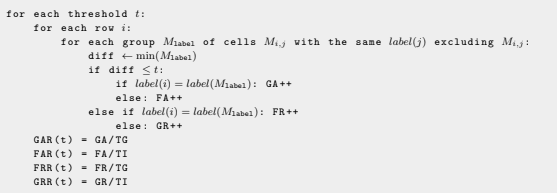
\includegraphics[width=5in]{imgs/verifica-mt.PNG}
    \caption{}
    \label{fig:verifica-mt}
\end{figure}

\paragraph{Identificazione, open-set template multipli} ogni riga è un set di 2 operazioni, uno da impostore e uno da genuino.

\begin{figure}[H]
    \centering
    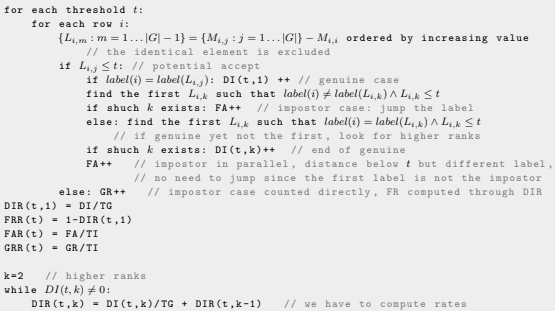
\includegraphics[width=5in]{imgs/identificazione-mt1.PNG}
    \caption{}
    \label{fig:identificazione-mt}
\end{figure}

Per ottenere informazioni riguardo il CMS, possiamo utilizzare il seguente algoritmo dove, ogni riga è un'operazione da genuino (zero impostori, in quanto non usiamo alcuna threshold)

\begin{figure}[H]
    \centering
    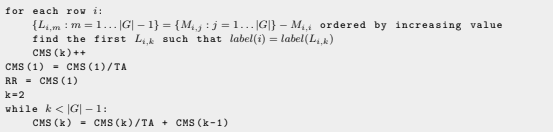
\includegraphics[width=5in]{imgs/identificazione-mt2.PNG}
    \caption{}
    \label{fig:verifica-st}
\end{figure}

Questi stessi algoritmi possono essere riutilizzati per una valutazione All probe vs All gallery, in quanto sulle righe abbiamo i probe e sulle colonne i template della gallery quindi è facile simularne la distribuzione.

\section{Definizione di metrica}
E' una funzione 
$$d: X \times X \rightarrow \mathbb{R}$$
dalle seguenti proprietà:
\begin{itemize}
    \item $d(x,y) \geq 0$
    \item $d(x,y) = 0 \iff x = y$
    \item $d(x,y) = d(y, x)$
    \item $d(x,z) \leq d(x,y) + d(y,z)$ (una semimetrica non ha questa proprietà)
\end{itemize}

Se non è simmetrica possiamo usare $$d^*(x,y) = \frac{d(x,y) + d(y,x)}{2}$$

\section{Affidabilità del riconoscimento (Recognition Reliability)}
\subsection{Doddington Zoo}
Doddington ha definito alcune similitudini con le classi animali per quanto riguarda lo speaker recognition:
\begin{itemize}
    \item \textbf{Pecora}: produce tratti biometrici che matchano bene con altri template di se stesso e male con quelli di altri soggetti (classe media)
    \item \textbf{Capra}: produce tratti biometrici che matchano poco con altri template di se stesso, aumentando così i casi di FR
    \item \textbf{Agnello}: produce tratti biometrici che sono facilmente riproducibili da altri, aumentando così i casi di FA nei suoi confronti
    \item \textbf{Lupo}: produce un matching score più alto rispetto alla media quando viene confrontato con template diversi dal suo, aumentando così i FA
\end{itemize}

Successivamente Yager ha individuato altre 4 classi, prendendo però in considerazione sia score genuini ($G_k$) che score impostori ($I_k$), al contrario di Doddington che invece prendeva in considerazione solo uno dei due. Ha individuato quindi:
\begin{itemize}
    \item \textbf{Camaleonte}: ha sia $G_k$ che $I_k$ alti, quindi riesce facilmente ad apparire simile ad altri. Può produrre tanti FA ma pochi FR
    \item \textbf{Fantasma}: ha sia $G_k$ che $I_k$ bassi, quindi causa tanti FR
    \item \textbf{Colomba}: è un'estensione della pecora di Doddington, ha $G_k$ alto e $I_k$ basso, quindi è l'utente ideale.
    \item \textbf{Verme}: avendo $G_k$ basso e $I_k$ alto è il peggiore utente che si possa avere.
\end{itemize}

\subsection{Misurare la qualità di un sample}
I sample presi in input possono avere una qualità diversa (per diversi motivi, es.: qualità sensore, tempo, ombre, etc..), possiamo quindi definire delle misure di affidabilità del riconoscimento che ci aprono ulteriori opzioni come ad esempio il richiedere all'utente di ripetere la cattura del sample.

\subsubsection{Qualità dell'immagine}
Una possibile misura di qualità è tramite la stima della qualità dell'immagine. Questa può essere effettuata in diversi modi:
\begin{itemize}
    \item Prendendo tutte le immagini in $TR$ e calcolando un \textbf{template medio} da utilizzare come \textbf{riferimento}.
    \item Stimando la \textbf{nitidezza dell'immagine} andando a visualizzare l'istogramma delle frequenze; una mancanza di alte frequenze significa una bassa nitidezza (immagine sfocata)
    \item Nel caso di un face recognizer:
    \begin{itemize}
        \item $SP$ per misurare la distorsione rispetto a una posa frontale, misuriamo quindi dei disallineamenti sui vari assi di rotazione. $$SP = \alpha (1-roll) + \beta (1-yaw) + \gamma (1-pitch)$$
        \item $SI$ per misurare l'omogeneità dei livelli di grigio in alcune zone predeterminate della faccia, utile per vedere se ci sono ombre nette in alcuni punti. $$SI = 1 - F(std(mc))$$
        \item $SY$ per misurare la simmetria della faccia $$SY = \sum_{(i,j) \in X} sym(P_i, P_j)$$
    \end{itemize}
\end{itemize}

Visualizzando la \textbf{distribuzione di un dataset rispetto alle misure proposte/scelte} è possibile decidere \textbf{quali sample scartare} (possibilmente solo quelli che presentano gravi distorsioni), sapendo a priori quanto questo inciderà sulla grandezza finale del dataset. Per valutare le performance di una misura di qualità possiamo verificare l'aumento o la diminuzione delle performance del modello finale (\textit{EER}): una buona misura di qualità dovrebbe aumentare l'efficacia del modello sui sample con score alti.

\begin{figure}[H]
    \centering
    \subfloat[Distribuzione di vari dataset rispetto alle misure proposte]{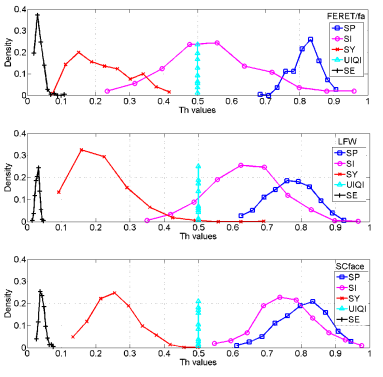
\includegraphics[width=2.5in]{imgs/qm1.PNG}}
    \subfloat[Performance di un sistema in seguito all'uso di misure di qualità]{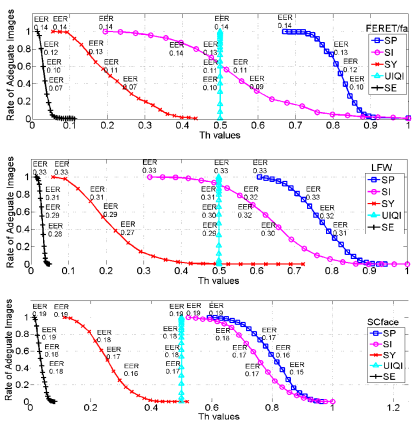
\includegraphics[width=2.5in]{imgs/qm2.PNG}}
    \caption{}
    \label{fig:qm}
\end{figure}

Un altro approccio è tramite il concetto di ``\textbf{margine}", che viene calcolato nel seguente modo:
$$M(t) = |FAR(t) - FRR(t)|,$$ da notare che $M(t)=0$ se siamo sull'EER.

\subsection{SRR - System Response Reliability}
C'è una netta differenza tra misurare la qualità di un'immagine in input rispetto al misurare l'affidabilità di una risposta da parte del sistema.

\bigskip
Quest'ultimo approccio viene chiamato indice SRR, ovvero un valore nel range $[0,1]$ che fornisce una misura di quanto un sistema, in fase di identificazione, riesce a separare bene soggetti genuini da soggetti impostori sulla base di un singolo probe. Questo sistema utilizza una funzione $\varphi$ che misura la quantità di ``confusione" tra i possibili candidati: presa la lista data in output da una fase di identificazione, si guarda nell'intorno del risultato a rango 1. Se i soggetti a ranghi più bassi sono molto vicini, avremo una risposta poco affidabile, altrimenti se c'è una buona distanza avremo una risposta affidabile. Possibili esempi di $\varphi$ sono:
\begin{itemize}
    \item $$\varphi(p) = \frac{F(d(p, g_1)) - F(d(p, g_2))}{F(d(p, g_{|G|}))}$$
    \item $$\varphi(p) = 1 - \frac{|N_b|}{|G|}$$ dove $N_b = \{g_i \in G | F(d(p, g_i)) < 2F(d(p, g_1)) \}$
\end{itemize}

Definiamo poi $\varphi_k$, come quel valore che minimizza gli errori di $\varphi(p)$, ovvero i casi in cui, probe impostori hanno $\varphi(p_I) > \varphi_k$ e probe genuini hanno $\varphi(p_G) \leq \varphi_k$. Valori $\varphi(p)$ molti distanti da $\varphi_k$ avranno un SRR maggiore, quindi:
\[
S(\varphi(p), \varphi_k) =
\begin{cases}
1-\varphi_k  & \text{se $\varphi(p)>\varphi_k$,} \\
\varphi_k & \text{altrimenti} 
\end{cases}
\]
e $$SRR = \frac{\varphi(p) - \varphi_k}{S(\varphi(p), \varphi_k)}$$

\subsection{Aggiornamento dei template}
Un altro modo per aumentare la qualità e l'affidabilità di un sistema è quella tramite l'aggiornamento dei template (evitando problemi come l'invecchiamento). Questa operazione per una maggiore sicurezza deve essere fatta in soli due possibili modi:
\begin{itemize}
    \item Supervisionata (supervised)
    \item Semi-supervisionata (semi-supervised)
\end{itemize}

\section{Riconoscimento facciale}
I fattori più importanti di un sistema biometrico sono l'\textbf{accettabilità}, l'\textbf{affidabilità} e l'\textbf{accuratezza}. Il \textbf{DNA}, ad esempio, fornisce un'alta accuratezza e affidabilità ma una bassa accettabilità, in quanto il metodo di prelievo è sicuramente intrusivo. Le \textbf{impronte digitali}, invece, forniscono anch'esse buone prestazioni, ma possono spesso presentarsi in modo ``parziale" e inoltre sono spesso associate ai "criminali". Il \textbf{riconoscimento facciale} invece è altamente accettato, in quanto siamo abituati a farci foto e a pubblicarle, ma l'accuratezza può diminuire drasticamente in casi non controllati. Possibili problemi relativi a essa sono:
\begin{itemize}
    \item A-PIE: invecchiamento, posa, illuminazione ed espressione
    \item Facilmente camuffabile: makeup, chirurgia plastica, occhiali, etc..
    \item Variazione intra-personale e similarità inter-personale
\end{itemize}

La struttura generale di un riconoscitore facciale prevede: 
$$\text{cattura immagine} \rightarrow \text{localizzazione, crop, normalizzazione} \rightarrow \text{estrazione feature}$$

\subsection{Localizzazione della faccia}
L'obiettivo qui è quello di contare quante facce ci sono all'interno di un'immagine e successivamente individuarne la posizione, indipendentemente da A-PIE e sfondo.

Possiamo avere approcci di diversa natura:
\begin{itemize}
    \item \textbf{Basati su feature}: si individuano le feature principali di una faccia (ad esempio posizione occhi, posizione naso, etc..) e poi si possono verificare diverse proprietà di queste (es.: colore della pelle corretto o distanza tra naso e occhi entro una certa soglia)
    \item \textbf{Basati su immagine}: solitamente vengono utilizzati dei modelli di machine learning che imparano da immagini esemplificative.
\end{itemize}

\subsubsection{Algoritmo A}
Vediamo un primo esempio di algoritmo per localizzare una faccia ideato da Hsu.
E' composto dai seguenti step:
\begin{enumerate}
    \item Ricerca di possibili facce
    \begin{enumerate}
        \item Aggiustamento dell'illuminazione, in quanto il colore della pelle varia in base all'illuminazione dell'ambiente
        \item Passaggio a uno spazio di colori diverso da RGB, ovvero $Y, C_b, C_r$
        \item Localizzazione in base al modello della pelle, che può essere creato ad esempio tramite K-Means, e successiva connessione delle componenti individuate da questo modello.
    \end{enumerate}
    \item Verifica delle possibili facce individuate, tramite l'individuazione delle feature facciali (occhi e naso).
    \item Assegnamento di uno score basato sulle possibili combinazione di occhi e naso e scelta del triangolo con score maggiore (e superiore a una certa soglia).
    \item Individuazione dei contorni della faccia tramite Hough.
\end{enumerate}

\subsubsection{Algoritmo B}
Viola Jones rappresenta una vera e propria innovazione per quanta riguarda la localizzazione
di una faccia all'interno di un'immagine. Essendo l'algoritmo basato su machine learning, il training di questo è avvenuto utilizzando un dataset personalizzato nel quale vengono etichettate immagini come positive, nel caso in cui ci sia una faccia e come negative nel caso in cui non ve ne sia alcuna.

\bigskip
Le idee utilizzate dietro questo algoritmo sono sostanzialmente:
\begin{itemize}
    \item Utilizzo di \textbf{Haar feature} con valutazione veloce tramite integrazione di immagini: vengono calcolate su una sotto-regione di una sotto-finestra di un'immagine, andando a calcolarne il valore tramite la seguente formula
    $$Value = \sum \text{valore dei pixel nell'area bianca } - \sum \text{valore dei pixel nell'area nera}$$
    \item \textbf{Ada-Boosting} per la selezione di feature: vengono creati diversi weak-classifier, uno per feature, e tramite adaptive boosting riusciamo a creare uno strong classifier composto da un subset di weak-classifier.
    \item \textbf{Classificatori a cascata} per velocizzare l'algoritmo: vengono creati diversi strong classifier, ognuno dei quali viene messo a cascata.
\end{itemize}

\section{Riconoscimento facciale 2D}
Nel riconoscimento facciale 2D abbiamo principalmente due problematiche da risolvere:
\begin{itemize}
    \item Costruzione di feature discriminative e rappresentative
    \item Costruzione di un classificatore che possa generalizzare anche su oggetti mai visti nel training
\end{itemize}

In questo caso quindi ci troviamo a rappresentare le facce all'interno di immagini digitali, che vengono rappresentate da matrici a due dimensioni ($w\times h$) oppure vettori unidimensionali ($d=w\times h$). L'alta dimensionalità dei dati (es.: immagine $100 \times 100$ ha dimensione $10000$) ci porta subito a un primo problema, ovvero il ``\textbf{Curse of dimensionality}".
Quando la dimensionalità aumenta, il volume dello spazio aumenta così velocemente che i dati diventano sparsi/radi. 
La sparsità dei dati, nel momento in cui vengono utilizzati strumenti statistici come ad esempio i modelli di machine learning, diminuisce drasticamente la capacità predittiva di questi in quanto si hanno bisogno di tanti più esempi per generalizzarne le regole predittive.

\subsection{PCA - Principal Component Analysis}
Una possibile soluzione al curse of dimensionality è data da PCA, ovvero un metodo statistico che ci consente di ridurre l'alta dimensionalità di uno spazio (es. $N$) mappando i dati in un altro spazio con una dimensionalità decisamente più piccola (es. $K << N$) minimizzando la perdita di informazioni.

Ciò che viene fatto sostanzialmente è individuare dei nuovi assi, ortogonali tra loro, su cui proiettare i dati che però ne massimizzano la varianza. L'ortogonalità di questi ci permette di escludere componenti correlate tra loro che risultano quindi ridondanti.

\bigskip
Nella pratica vengono calcolati due elementi:
\begin{enumerate}
    \item Elemento medio del training set $\Bar{x}$
    $$\Bar{x} = \frac{1}{m} \sum_{i=1}^{m} x_i$$
    \item Matrice di covarianza $C$ ($n \times n$)
    $$C = \frac{1}{m} \sum_{i=1}^{m} (x_i - \Bar{x})(x_i - \Bar{x})^T $$
\end{enumerate}
La nuova dimensione $k$ è data dalla matrice di proiezione dove le colonne sono i $k$ autovettori di $C$, corrispondenti ai $k$ autovalori di $C$. Plottando gli autovalori possiamo ottenere la varianza lungo gli autovettori.

\bigskip
PCA però ha dei lati negativi:
\begin{itemize}
    \item Mancanza di potere discriminativo
    \item In presenza di variazioni PIE, il modello potrebbe utilizzare quelle come componenti principali (feature inutile)
\end{itemize}

\subsection{LDA - Linear Discriminant Analysis}
Alcuni dei problemi di PCA possono essere dati dal fatto che lavoriamo su dati in una maniera unsupervised (non supervisionata), ovvero senza tenere in considerazione le classi dei vari sample. Una soluzione supervised è proposta da LDA, ovvero un metodo simile a PCA ma che minimizza la distanza intra-classe e cerca di massimizzare invece la distanza tra classi.


\subsection{Estrattori di feature}
Le feature rilevanti di un'immagine possono estratte tramite l'utilizzo di \textbf{filtri}, \textbf{trasformazioni} o diversi \textbf{operatori} ognuno designato e utilizzato per uno specifico obiettivo. Di seguito verranno riportati a titolo esemplificativo solo alcuni di questi in quanto ne esistono centinaia.

\bigskip
Ovviamente in caso di alta dimensionalità delle feature potremmo (o forse dovremmo) ricorrere ai metodi di riduzione della dimensionalità descritti nella sezione precedente.
\paragraph{Gabor filter}
E' un filtro lineare utilizzato in applicazioni di edge detection, analisi di texture e estrazione di feature, e si pensa che sia simile al sistema percettivo visivo di noi umani.
Un Gabor filter 2D non è altro che un kernel Gaussiano modulato da un'onda piana sinusoidale.

\bigskip
E' possibile creare diversi Gabor filter andando a cambiare i seguenti parametri:
\begin{itemize}
    \item $\lambda$: frequenza, controlla lo spessore della striscia; più è grande più sarà spessa.
    \item $\theta$: orientamento, controlla la rotazione della striscia ed è espresso come un angolo.
    \item $\gamma$: aspect ratio, controlla l'altezza della striscia; più è grande più l'altezza diminuirà.
    \item $\sigma$: larghezza di banda, controlla la scala generale determinando anche il numero di strisce; aumentando questo valore avremo più strisce con meno distanza tra loro.
\end{itemize}

\begin{figure}[H]
    \centering
    \subfloat[Lambda]{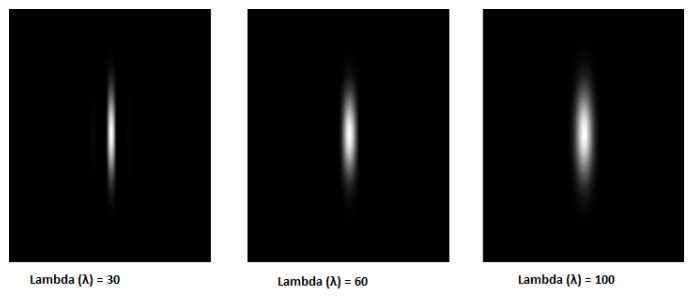
\includegraphics[width=4in]{imgs/lambdagabor.PNG}}\\
    \subfloat[Theta]{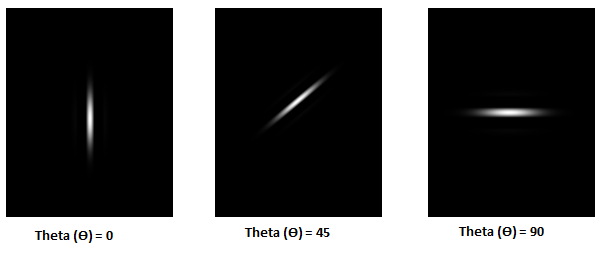
\includegraphics[width=4in]{imgs/thetagabor.PNG}}\\
    \subfloat[Gamma]{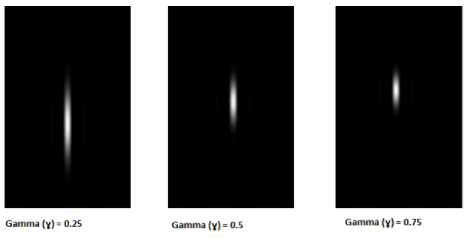
\includegraphics[width=4in]{imgs/gammagabor.PNG}}\\
    \subfloat[Sigma]{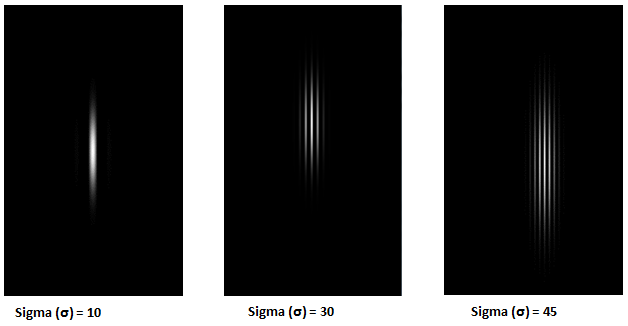
\includegraphics[width=4in]{imgs/sigmagabor.PNG}}
    \caption{}
    \label{fig:gaborEg}
\end{figure}

Ovviamente in immagini o task complessi con un solo gabor filter non è possibile individuare le feature discriminanti, ciò che possiamo fare è utilizzare un'insieme di filtri (bank of filters) che ci aiutino a creare un vettore di feature. Ovvero, applicando un filtro su un'immagine otterremo in output una nuova immagine che può essere ``appiattita" e utilizzata come vettore di feature.

\begin{figure}[H]
    \centering
    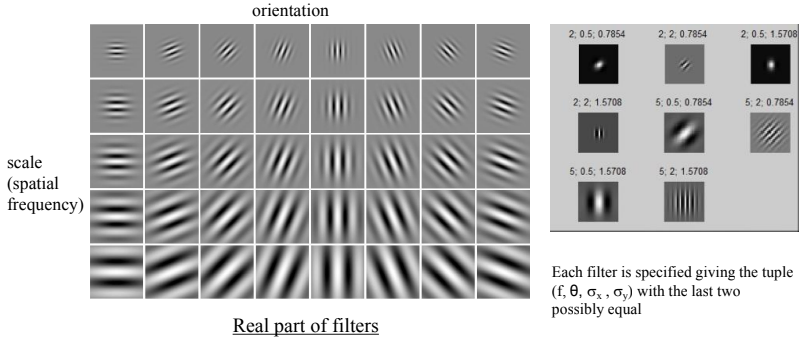
\includegraphics[width=4in]{imgs/gabor filter.PNG}
    \caption{Esempio di ``banca di filtri"}
    \label{fig:gaborFilters}
\end{figure}

Questa procedura, su immagini molto grandi, porta ad un'alta dimensionalità; possibili soluzioni sono:
\begin{itemize}
    \item Applicare il filtro su un subset di pixel, come ad esempio una griglia $\implies$ dimensionalità ridotta, ma possibile perdità di informazioni salienti (dovuta a possibili rotazioni ad esempio)
    \item Applico il filtro su tutti i pixel, ma poi seleziono solo i punti con picchi di valori $\implies$ problemi di allineamento
\end{itemize}

\paragraph{EBGM - Elastic Bunch Graph Matching}
Questo metodo fa uso di grafi, nello spacifico abbiamo per ogni soggetto una collezione di grafi (per questo il nome ``\textbf{bunch}"), uno per ogni posa, dove:
\begin{itemize}
    \item I vertici sono pesati dalla distanza tra i nodi
    \item I nodi contengono un insieme di risultati di diversi gabor filter (in genere 5 differenti frequenze e 8 diversi orientamenti), conservati in questa struttura chiamata ``\textbf{Jet}", e sono posizionati in punti importanti come ad esempio naso, occhi e bocca. 
\end{itemize}

\paragraph{LBP - Local Binary Pattern}
E' un operatore che lavora pixel per pixel che ci aiuta ad estrarre informazioni riguardo le texture all'interno di un'immagine (proprio per questo può essere utilizzato anche per antispoofing). Nella sua prima versione va a considerare una griglia di vicini $3\times 3$ dove a ognuno dei quali viene assegnato un valore binario: se il suo valore era maggiore del valore del pixel centrale veniva assegnato 1 altrimenti 0. Effettuando questa operazione con un ordine di processo dei vicini fisso (es.: partendo dal vicino in alto a sinistra) si ottiene una stringa binaria, il quale valore, convertito in decimale, viene assegnato al pixel centrale.

\bigskip
Questa versione è stata poi generalizzata andando a parametrizzare il numero di punti vicini ($P$) e il loro raggio di distanza ($R$), producendo così la seguente formula:
$$LBP_{R,P} = \sum_{i=0}^{P-1} sign(p_i - p_c)2^P$$

Un pattern viene definito \textbf{uniforme} se nella stringa binaria contiene al massimo due transizioni $0 \rightarrow 1$, $1 \rightarrow 0$. Questi rappresentando le informazioni essenziali (la maggior parte dei valori assunti dalla stringa binaria sono dati da stringhe NON uniformi), ci consentono di ridurre notevolmente il numero di punti da considerare riducendo la dimensionalità.

\bigskip
Vediamo ora come possiamo ottenere un vettore di features:
\begin{itemize}
    \item L'immagine viene suddivisa in sotto-finestre grandi $k\times k$
    \item Per ogni sotto-finestra calcoliamo un istogramma (ad ogni bin corrisponde un pattern)
    \item Il vettore finale viene costruito concatenando i $k^2$ istogrammi.
\end{itemize}

\textbf{Nota:} le rotazioni variano i risultati di \textit{LBP}. Una possibile soluzione è quella di effettuare diversi shift logici verso destra della stringa binaria e prendere sempre il valore (decimale) minimo.

\subsection{Classificazioni di sistemi di riconoscimento facciale}
\begin{itemize}
    \item \textbf{Metodi basati sull'apparenza della faccia}: PCA, LDA, alcune reti neurali; utilizzano l'immagine per intero e quindi non perdono informazioni da subito concentrandosi su regioni specifiche. Gli svantaggi sono dati dal fatto che danno la stessa importanza a ogni pixel, hanno bisogno di un'alta correlazione tra dati di training e test, su grandi variazioni PIE non performano così bene.
    \item \textbf{Metodi basati su feature locali}: EBGM, LBP; sono robusti a varianze di posizione in quanto vengono prima individuati i punti da cui estrarre le feature, e inoltre sono computazionalmente veloci. Come principale svantaggio hanno la scelta a priori dei punti da cui estrarre le feature (se i punti da cui estrarre le feature non sono molto discriminativi avremo sicuramente pessime performance)
    \item \textbf{Sistemi basati su grafi}: a ogni faccia è associato un grafo, dove ogni nodo corrisponde a dei punti discriminativi della faccia. Sono ottimi dal punto di vista di variazioni di posizione e illuminazione, ma purtroppo il training e il testing sono lunghissimi.
    \item \textbf{Sistemi basati su immagini termografiche}: sono ottimi per quanto riguarda variazioni di illuminazione, però purtroppo richiedono attrezzatura adeguata e la temperatura misurata può variare in base allo stato del soggetto. Sono inoltre sensibili ai movimenti. 
\end{itemize}

\section{Riconoscimento facciale 3D}
Nel riconoscimento facciale 2D i problemi che occorrono sono dovuti soprattutto a variazioni A-PIE e a possibili travestimenti da parte di impostori. Con il riconoscimento 3D molti di questi problemi non sono più tali (posizione e espressione possono essere corretti ad esempio), introducendo però altre complicanze come una maggiore complessità di acquisizione e una maggiore complessità nello gestire i dati acquisiti. Possibili rappresentazioni sono:
\begin{itemize}
    \item \textbf{2.5D}: solitamente sono immagini 2D che, oltre a conservare l'informazione del colore nei 3 canali rgb, mantengono una quarta informazione che è la distanza d'acquisizione.
    \item \textbf{3D}: una serie di punti che connessi tra loro (solitamente tramite triangolarizzazione) formano un cosiddetto mesh 3D. I metodi di acquisizione sono diversi ognuno con i suoi pro e i suoi contro (camera stereoscopica, scanner di light pattern, laser scanner)
\end{itemize}

Il preprocessing che viene effettuato sui dati acquisiti può andare a risolvere i seguenti problemi:
\begin{itemize}
    \item Presenza di spike o rumore
    \item Presenza di ``buchi" nel mesh: smoothing gaussiano o interpolazione lineare aiutano a risolvere il problema
    \item Decentramento
\end{itemize}

\paragraph{Immagine 2D $\rightarrow$ 3D} Sfruttando le proprietà di shading, e quindi come la luce riflette su una superficie, o in particolare qui sulla nostra faccia, è possibile stimare informazioni come ad esempio la profondità e ricavare quindi così un mesh 3D di una faccia da un'immagine 2D (in realtà molte volte un'immagina sola non basta, è quindi necessario avere più immagini con più orientamenti della faccia).

\bigskip
Un'altra tecnica è il ``\textbf{morphing}", dove semplicemente viene creata una faccia 3D di riferimento e viene poi modellata per ottenere un risultato congruo a un'immagine di una persona. Questo ci permette di poter cambiare anche alcune caratteristiche del modello 3D così da poter stimare un modello sotto variazioni di espressione o età ad esempio.

\begin{figure}[H]
    \centering
    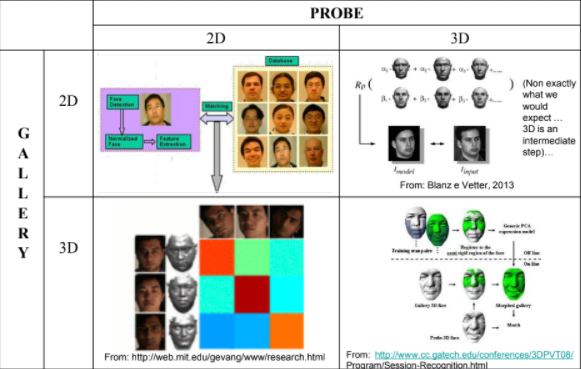
\includegraphics[width=4in]{imgs/2d3d.PNG}
    \caption{Possibili configurazioni}
    \label{fig:2d3dconf}
\end{figure}

Da un modello 3D ciò che possiamo fare è:
\begin{itemize}
    \item Aggiustare la posa
    \item Calcolare la normal map da confrontare con altre normal map
\end{itemize}

\section{Valutazione di un riconoscitore facciale}
Quando sviluppiamo un riconoscitore facciale (ma in generale un pattern recognizer) le classiche misure come FAR, FRR, CMS, etc.. forniscono una valutazione marginale del sistema; bisogna prendere in considerazione le variazioni (non solo le A-PIE) che ci possono essere e soprattutto il dataset scelto può condizionare i risultati.

Proprio per questo motivo \textbf{FERET} è stato il primo dataset messo a disposizione di tutti e utilizzato come strumento di benchmark dei propri face recognizer.


\section{Spoofing e Camuffamento}
Lo \textbf{spoofing} consiste nell'ingannare un sistema biometrico assumendo un'identità che non ci appartiene.
La differenza sostanziale tra spoofing e \textbf{camuffamento} (camouflage) è data dal fatto che nel primo l'obiettivo è essere riconosciuti con un'altra identità e quindi ottenere un genuine accept; nel secondo invece l'obiettivo è quello di non far riconoscere al sistema la propria identità (es.: un criminale che non vuole farsi riconoscere dalle telecamere di sicurezza).

\bigskip
Questo tipo di attacco può avvenire in diversi punti del sistema e possiamo classificarli in due modi:
\begin{enumerate}
    \item \textbf{Diretto}: avviene direttamente al momento dell'acquisizione
    \item \textbf{Indiretto}: avviene nelle fasi successive della pipeline
\end{enumerate}

\subsection{Spoofing del volto}
Per quanta riguarda un face recognizer possono avvenire i seguenti attacchi:
\begin{itemize}
    \item \textbf{Print attack}: è un attacco diretto dove viene presentata un'immagine (in forma stampata o su display) del soggetto da identificare. Questo tipo di attacco può essere identificato abbastanza facilmente andando a sfruttare le differenze che ci sono tra un'immagine di una faccia catturata da due dispositivi (foto stampata e ricatturata dal sensore del sistema biometrico) e una catturata una singola volta. Tra queste differenze nominiamo la differenza dei possibili colori, differenza di come la luce riflette, differenza tra le texture. In tutti questi casi LBP viene in nostro aiuto. Un altro metodo consiste nell'individuare gesti involontari che ci danno informazioni riguardo la liveness di un soggetto, come ad esempio il battito delle ciglia.
    \item \textbf{Video}: simile al precedente ma viene presentato un video del soggetto da identificare. Anche qui LBP viene utilizzato.
    \item \textbf{Maschera facciale}: viene prodotta una maschera 3D, queste hanno un notevole costo e quindi sono meno frequenti. Una possibile soluzione è quella di verificare come la luce riflette sulla pelle (su una maschera in plastica la luce ad esempio rifletterà, mentre sulla pelle viene assorbito)
\end{itemize}

Quando produciamo un sistema biometrico, se prendiamo in considerazione anche gli attacchi di spoofing dobbiamo utilizzare una metrica diversa dal classico FAR, ovvero \textbf{Spoofing-FAR}, che prende in considerazione anche i possibili impostori che vengono accettati grazie allo spoofing.

Per la valutazione del sistema di spoofing invece possiamo usare:
\begin{itemize}
    \item \textbf{False Living Rate} (FLR): numero di casi di soggetti che sono stati additati come ``reali" dal sistema di spoofing ma in realtà erano fake.
    \item \textbf{False Fake Rate} (FFR): numero di casi di soggetti che sono stati additati come ``fake" ma erano reali.
\end{itemize}

\section{Riconoscimento dell'orecchio}
L'orecchio è un tratto biometrico composto da una sua struttura ben definita:
\begin{itemize}
    \item \textbf{Helix}: il bordo esterno
    \item \textbf{Anti-Helix}: i ``bordi" interni
    \item \textbf{Lobo}
    \item \textbf{Tacca intratragica}: è il punto tra il lobo e il foro dell'orecchio 
\end{itemize}

Vediamo i lati positivi e negativi:
\begin{itemize}
    \item Pro: è un tratto passivo, non varia con gli anni, solitamente non è coperto, non sono richieste alte risoluzioni, non è affetto da variazioni dell'espressione
    \item Contro: sensibile a variazioni di illuminazione e posa
\end{itemize}

Una prima prova dell'universalità e unicità di questo tratto è molto recente: 1989 da Iannarelli, purtroppo però l'indagine è stata effettuata campionando pochissimi esempi.
Iannarelli ha poi classificato le orecchie in 4 possibili forme esterne: triangolari, circolari, rettangolari e ovali.

\subsection{Localizzazione dell'orecchio}
Principalmente abbiamo 3 modi:
\begin{itemize}
    \item \textbf{Individuazione di punti di interesse}: possono estratti in diversi modi, un esempio è tramite reti neurali, da notare che qui siamo interessati solo all'estrazione dei punti, quindi possiamo lavorare anche su immagini a bassa risoluzione. Una volta individuati i punti di interesse, questi vengono usati come riferimento per andare a creare il rettangolo che conterrà l'orecchio (che possiamo normalizzare)
    \item \textbf{Object detection}: possiamo utilizzare un object detector come ad esempio viola-jones
    \item \textbf{Cattura della distanza}: può essere utilizzata un'immagine che comprende anche la misura della distanza. L'orecchio conterrà le componenti con distanza minore.
\end{itemize}

\subsection{Estrazione feature e riconoscimento}

\subsubsection{2D}
Possiamo avere i seguenti approcci:
\begin{itemize}
    \item Iannarelli: dove viene identificato il punto di origine dell'helix e viene usato come punto di partenza di 4 segmenti su cui effettuare 12 misurazioni. Il vettore di feature contiene info come il gender, l'etnicità e le 12 misurazioni. Il problema di questo approccio è che se il punto di origine è errato, tutta la misurazione è errata.
    \item Diagramma Voronoi
    \item Campi di forza: basati su proprietà fisiche dove ogni pixel viene considerato come un ``attrattore"
    \item Jet
    \item SIFT
\end{itemize}

\subsubsection{3D} In questo caso vengono valutati fattori come profondità e curvatura delle varie componenti di un orecchio.

\subsubsection{Camera termica}
\begin{itemize}
    \item Pro: facile individuare l'orecchio, robusto a occlusioni
    \item Contro: sensibile a movimenti, bassa risoluzione, costo alto
\end{itemize}

\section{Riconoscimento dell'iride}
L'iride è una membrana muscolare bucata dalla pupilla che, data la sua alta randotipicità la rende un ottimo tratto biometrico, c'è comunque una piccola traccia di tratti ereditati ma si parla di eredità a 4 generazioni di distanza e quindi può creare problemi solo in casi eccezionali. 

Tra i \textbf{vantaggi} abbiamo: alto potere discriminativo, cattura non invasiva e non varianza nel tempo.

\medskip

Tra gli \textbf{svantaggi} invece: catturare sample di qualità richiede una buona attrezzatura e inoltre può risultare scomoda.

\bigskip

La cattura può avvenire:
\begin{itemize}
    \item \textbf{Luce visibile}: la luce viene riflessa dall'iride generando ``rumore" e rovinando la qualità del sample. Una basse illuminazione invece non permette di catturare bene i tratti dell'iride e quindi è richiesta una fase di preprocessing.
    \item \textbf{NIR}: la maggior della luce viene assorbita, questo permette di catturare molti più dettagli soprattutto su iridi molto scure. Come contro abbiamo che è richiesta un'apparecchiatura specifica e perdiamo informazione sul colore dell'iride.
\end{itemize}

\subsection{Sistema di Daugmann}
\textit{Daugmann} è stato uno dei pionieri dei metodi di riconoscimento tramite iride e il suo sistema prevedeva le seguenti fasi:
\begin{itemize}
    \item Localizzazione
    \item Normalizzazione
    \item Estrazione di feature (coding)
    \item Matching
\end{itemize}

\paragraph{Localizzazione} Per localizzare i due cerchi del limbo e della pupilla, Daugmann fa uso dell'operatore integro-differenziale che funge da ``edge detector circolare": l'operatore cerca percorsi circolari nei quali la varianza dei pixel viene massimizzata, variando la posizione e il raggio del cerchio che stiamo cercando.

Per la localizzazione delle palpebre avviene un procedimento analogo dove viene utilizzato un operatore simile ma che cerca archi anzichè cerchi.

\paragraph{Normalizzazione}
Normalizzare le iridi segmentate è importante in quanto ci permette di lavorare su un piano lineare dove ogni iride assume la stessa dimensione, indipendentemente dalla grandezza dei cerchi individuati.
Ciò che viene usato da Daugmann è il \textbf{Rubber Sheet Model}, ovvero un modello di mapping pseudo-polare. La differenza con un mapping polare classico sta nel fatto che qui si cerca di correggere un possibile decentramento tra pupilla e limbo (dovuta ad esempio a una variazione dello sguardo) andando a utilizzare come raggio il segmento tra il cerchio della pupilla e il cerchio del limbo (per ogni angolo potremmo avere raggi più o meno lunghi), prendendo poi un numero finito di punti lungo questo.

\paragraph{Coding e matching}
Applica una serie di \textbf{gabor filter} per ottenere poi un'immagine binaria. Per il matching invece utilizza la \textbf{hamming distance}.


\subsection{NICE}
Il sistema di Daugmann funziona molto bene in casi di acquisizione controllata e con acqusizione NIR. E' stata quindi iniziata una challenge chiamata NICE - Noisy Iris Challenge Evalutaion, articolata in due fasi
\begin{enumerate}
    \item \textbf{ NICE I}: valutato su segmentazione dell'iride e individuazione e correzione di noise
    \item \textbf{NICE II}: valutato sulla parte di encoding e matching
\end{enumerate}

In NICE II, il gruppo italiano \textit{BIPLAB} è arrivato sesto proponendo un approccio all'encoding basato su LBP (per l'estrazione delle regolarità della texture dell'iride) e BLOB (per l'estrazione delle singolarità).

\subsection{$IS_{IS}$}
$IS_{IS}$ è un algoritmo di segmentazione sviluppato dal gruppo di ricerca della professoressa M. De Marsico che si basa sui seguenti step:
\begin{enumerate}
    \item Segmentazione: viene applicato un filtro di posterizzazione per risaltare i contrasti nell'immagine e successivamente viene utilizzato canny edge detector per individuare dei possibili bordi. Successivamente viene utilizzato l'algoritmo di circle fitting di Taubin per individuare dei possibili cerchi candidati. I cerchi vengono poi selezionati in base ai loro score di \textbf{omogeneità} (solo per la pupilla) e \textbf{separabilità}.
    \item \textbf{Estrazione feature}: LBP + BLOB
\end{enumerate}

\section{Riconoscimento di impronte digitali}
Le impronte digitali sono state uno dei primi tratti biometrici ad essere utilizzate per identificare un soggetto, in particolare il primo approccio scientifico è dato da \textbf{Galton}, il quale ha dato una prima classificazione delle impronte digitali che definiamo come \textbf{macro singolarità} (archi, loop e spirali) e successivamente ha introdotto il concetto di minuzie che definiamo come \textbf{micro singolarità}; quest'ultime possono essere: \textit{punti di fine}, \textit{biforcazioni} e \textit{delta}.

\bigskip
In seguito un secondo approccio è quello di \textbf{Henry}, il quale ha proposto un'altra macro classificazione con la frequenza per ogni classe:
\begin{itemize}
    \item Spirali: 28\%
    \item Archi: 6.6\%
    \item Left Loop: 33.8\%
    \item Right Loop: 31.7\%
\end{itemize}

Le impronte digitali sono un tratto \textbf{randotipico}, ovvero vengono generate al momento della nascita e sono condizionate dall'ambiente e dalle superfici con le quali entra in contatto il feto. Questo garantisce un'alta univocità, anche se è stato osservato che tra gemelli, seppur le impronte siano diverse, sono comunque presenti delle similarità.

\subsection{AFIS - Automatic Fingerprint Identification System}
Il primo ente a collezionare impronte digitali è stata l'FBI, collezionando 10 impronte digitali, una per ogni dito, di diversi soggetti. Questo database crescendo esponenzialmente ha reso necessario l'intervento del calcolatore per verificare in modo automatico la similarità tra due impronte.

\subsection{Acquisizione}
L'acquisizione può avvenire principalmente secondo due modalità:
\begin{enumerate}
    \item \textbf{Offline}: consiste in due step, la prima è la creazione dell'impronta su carta tramite inchiostro ad esempio, con la successiva digitalizzazione dell'impronta ``stampata". In questa categoria rientrano le \textbf{impronte latenti}, ovvero quelle che lasciamo involontariamente sulle diverse superfici.
    \item \textbf{Online}: un solo step di acquisizione, in quanto viene utilizzato un sensore di cattura che digitalizza direttamente.
\end{enumerate}

Possibili problemi associati all'acquisizione sono:
\begin{itemize}
    \item Allineamento
    \item Condizioni della pelle non adatte
    \item Pressione del dito variabile
    \item Troppo movimento
    \item Parzialità dell'impronta latente
\end{itemize}

\subsection{Matching}
Gli esperti di analisi di impronte digitali consigliano di prendere in considerazione 4 aspetti:
\begin{itemize}
    \item Valutare prima un pattern globale (per scartare impronte con pattern diversi)
    \item Valutare la qualità, ovvero valutare le minuzie
    \item Valutare la quantità, ovvero ci deve essere un numero minimo di minuzie che matchano tra due impronte (consigliano almeno 12)
    \item Corrispondenza di dettagli che devono essere interconnessi
\end{itemize}

Di seguito vengono riportati dei possibili tipi di matching:
\begin{enumerate}
    \item Basato su correlazione: le due immagini vengono sovrapposte e viene fatto un calcolo della correlazione dei vari pixel (iterando sui possibili allineamenti). Ha un costo computazionale molto alto ed è sensibile a trasformazioni non lineari.
    \item Basato sulle ridge feature: utilizzato per immagini di bassa qualità quando quindi non è possibile estrarre le minuzie. Utilizza feature facili da estrarre come l'orientamento, la frequenza e la forma dei vari ridge. E' poco discriminativo.
    \item Basato su minuzie: vengono estratte le minuzie e vengono salvate come punti in uno spazio a due dimensioni. Il metodo poi cerca un possibile allineamento che massimizzi il numero di match di minuzie.
\end{enumerate}

\subsubsection{Segmentazione}
Si cerca di separare il background (isotropico) da ciò che è antisotropico, in questo caso le impronte. Isotropico significa che è indipendente dalla direzione (es.: ruotando uno sfondo bianco abbiamo sempre la stessa immagine).


\subsubsection{Macro features}
Una volta segmentata l'impronta possiamo iniziare a estrarre delle macro features come:
\begin{itemize}
    \item \textbf{Flusso dei ridge}: descritto da una directional map; si lavora su una griglia e non sull'immagine intera (quindi consideriamo i vicini di un certo pixel su questa griglia)
    \item \textbf{Densità dei ridge}: descritto da una density map.
\end{itemize}

Per estrarre le singolarità un metodo elegante è quello di utilizzare il \textbf{Poincarè index}, ovvero un valore che può assumere solo i seguenti valori:
\begin{itemize}
    \item 0 $\implies$ nessuna singolarità
    \item 180 $\implies$ loop
    \item -180 $\implies$ delta
    \item 360 $\implies$ spirale
\end{itemize}
E indica la rotazione totale dei vettori su una certa curva.

\subsubsection{Micro features}
Per estrarre le minuzie sono necessari i seguenti step:
\begin{enumerate}
    \item Binarizzazione dell'immagine
    \item Appiattimento dei ridge: i ridge vengono appiattiti a grandezza un 1 pixel
    \item Localizzazione delle minuzie: vengono individuati i pixel corrispondenti alle varie minuzie
\end{enumerate}

Per l'ultimo punto possiamo effettuare un'analisi del crossing number di un certo pixel $cn(p)$
$$cn(p) = \frac{1}{2} \sum_{i=1}^8 | val(p_{i\ mod\ 8}) - val(p_{i-1}) |$$

Se
\begin{itemize}
    \item $cn(p) = 0$: isola
    \item $cn(p) = 1$: terminazione
    \item $cn(p) = 2$: punto interno di un ridge
    \item $cn(p) = 3$: biforcazione
    \item $cn(p) > 3$: minuzia complessa
\end{itemize}

Un'altra feature che possiamo prendere in considerazione è la distanza tra minuzie espressa dal \textbf{ridge count}, ovvero il numero di ridge tra una minuzia e un'altra (solitamente i due punti scelti sono punti rilevanti)

\subsection{Approccio ibrido}
E' possibile utilizzare un approccio ibrido dove l'estrazione di minuzie aiuta a trovare il miglior allineamento possibile tra probe e template e poi utilizziamo una banca di gabor filter per l'estrazione delle feature. 

\subsection{Impronte finte}
E' facile creare delle possibili impronte artificiali con dei materiali come il silicone o gelatina, ma ogni materiale ha risposte diverse al sensore che stiamo utilizzando (e quindi potremmo capire se si tratta di un possibile attacco).
Per verificare la ``liveness" di un dito possiamo sfruttare ad esempio sensori che riescono a catturare lo scorrere del sangue.


\section{Approcci multibiometrici}
Gli approcci multibiometrici ci aiutano a contrastare attacchi di spoofing, in quanto l'attaccante dovrà bypassare più livelli. Per sistema multibiometrico possiamo intendere l'utilizzo di:
\begin{enumerate}
    \item più sensori di acquisizione
    \item più tratti biometrici (generalmente intendiamo questo)
    \item probe multipli
    \item algoritmi diversi
    \item istanze multiple
\end{enumerate}

La fusione di più tratti può avvenire in diversi punti:
\begin{itemize}
    \item A livello del \textbf{sensore}: in questo caso si utilizzano più acquisizioni da fondere in un unico modello
    \item A livello di \textbf{feature}: vengono fusi i vettori di feature. Potremmo avere problemi di dimensionalità (magari con dati ridondanti) e di incompatibilità.
    \item A livello di \textbf{score}: vengono fusi i punteggi, i quali a loro volta possono essere di 3 tipi:
    \begin{itemize}
        \item Astratto: viene restituita la classe del soggetto. In questo caso la fusione avviene tramite votazione, scegliendo la maggioranza. 
        \item Rank: viene restituita una lista dei rank per ogni classe. La fusione è possibile effettuarla tramite ``borda count". Supponiamo di avere $n$ classificatori e $k$ rank (quindi $k$ classi). Ogni classificatore produrrà la sua lista contenente i $k$ rank. Per ogni classe prendiamo i rank ottenuti dagli $n$ classificatori e li sommiamo. La classe con il valore più alto sarà quella restituita come risultato finale. 
        \item Misura: ogni classificatore da in output uno score basato su una misura. L'unica difficoltà qui è normalizzare i vari score in quanto probabilmente ognuno utilizzerà una misura diversa. Una volta fatto questo possiamo restituire lo score medio o, sapendo il livello di ``confidence" dei singoli classificatori, possiamo usare quel valore come peso per una somma pesata.
    \end{itemize}
    \item A livello di \textbf{decisione}: viene fusa la decisione booleana ``si/no". In questo possiamo o prendere l'AND di tutte le decisioni o l'OR. Un altro approccio è tramite voto a maggioranza. 
\end{itemize}
\end{document}
